\subsection{Architecture}

The suggested architecture in figure \ref{fig:suggestedArchitecture} only supports a handful of MIPS instructions, and lacks support for jump instructions that was present in the previous exercise.
However, by adding a shifter to the ALU and a few additional muxes, mainly to the memory stage, the number of supported instruction can be radically improved from 9 to 29.
The resulting architecture, which includes a forwarding unit for highly improved performance can be seen in figure \ref{fig:cpuArchitecture} below.

\begin{figure}[ht]
    \centering
    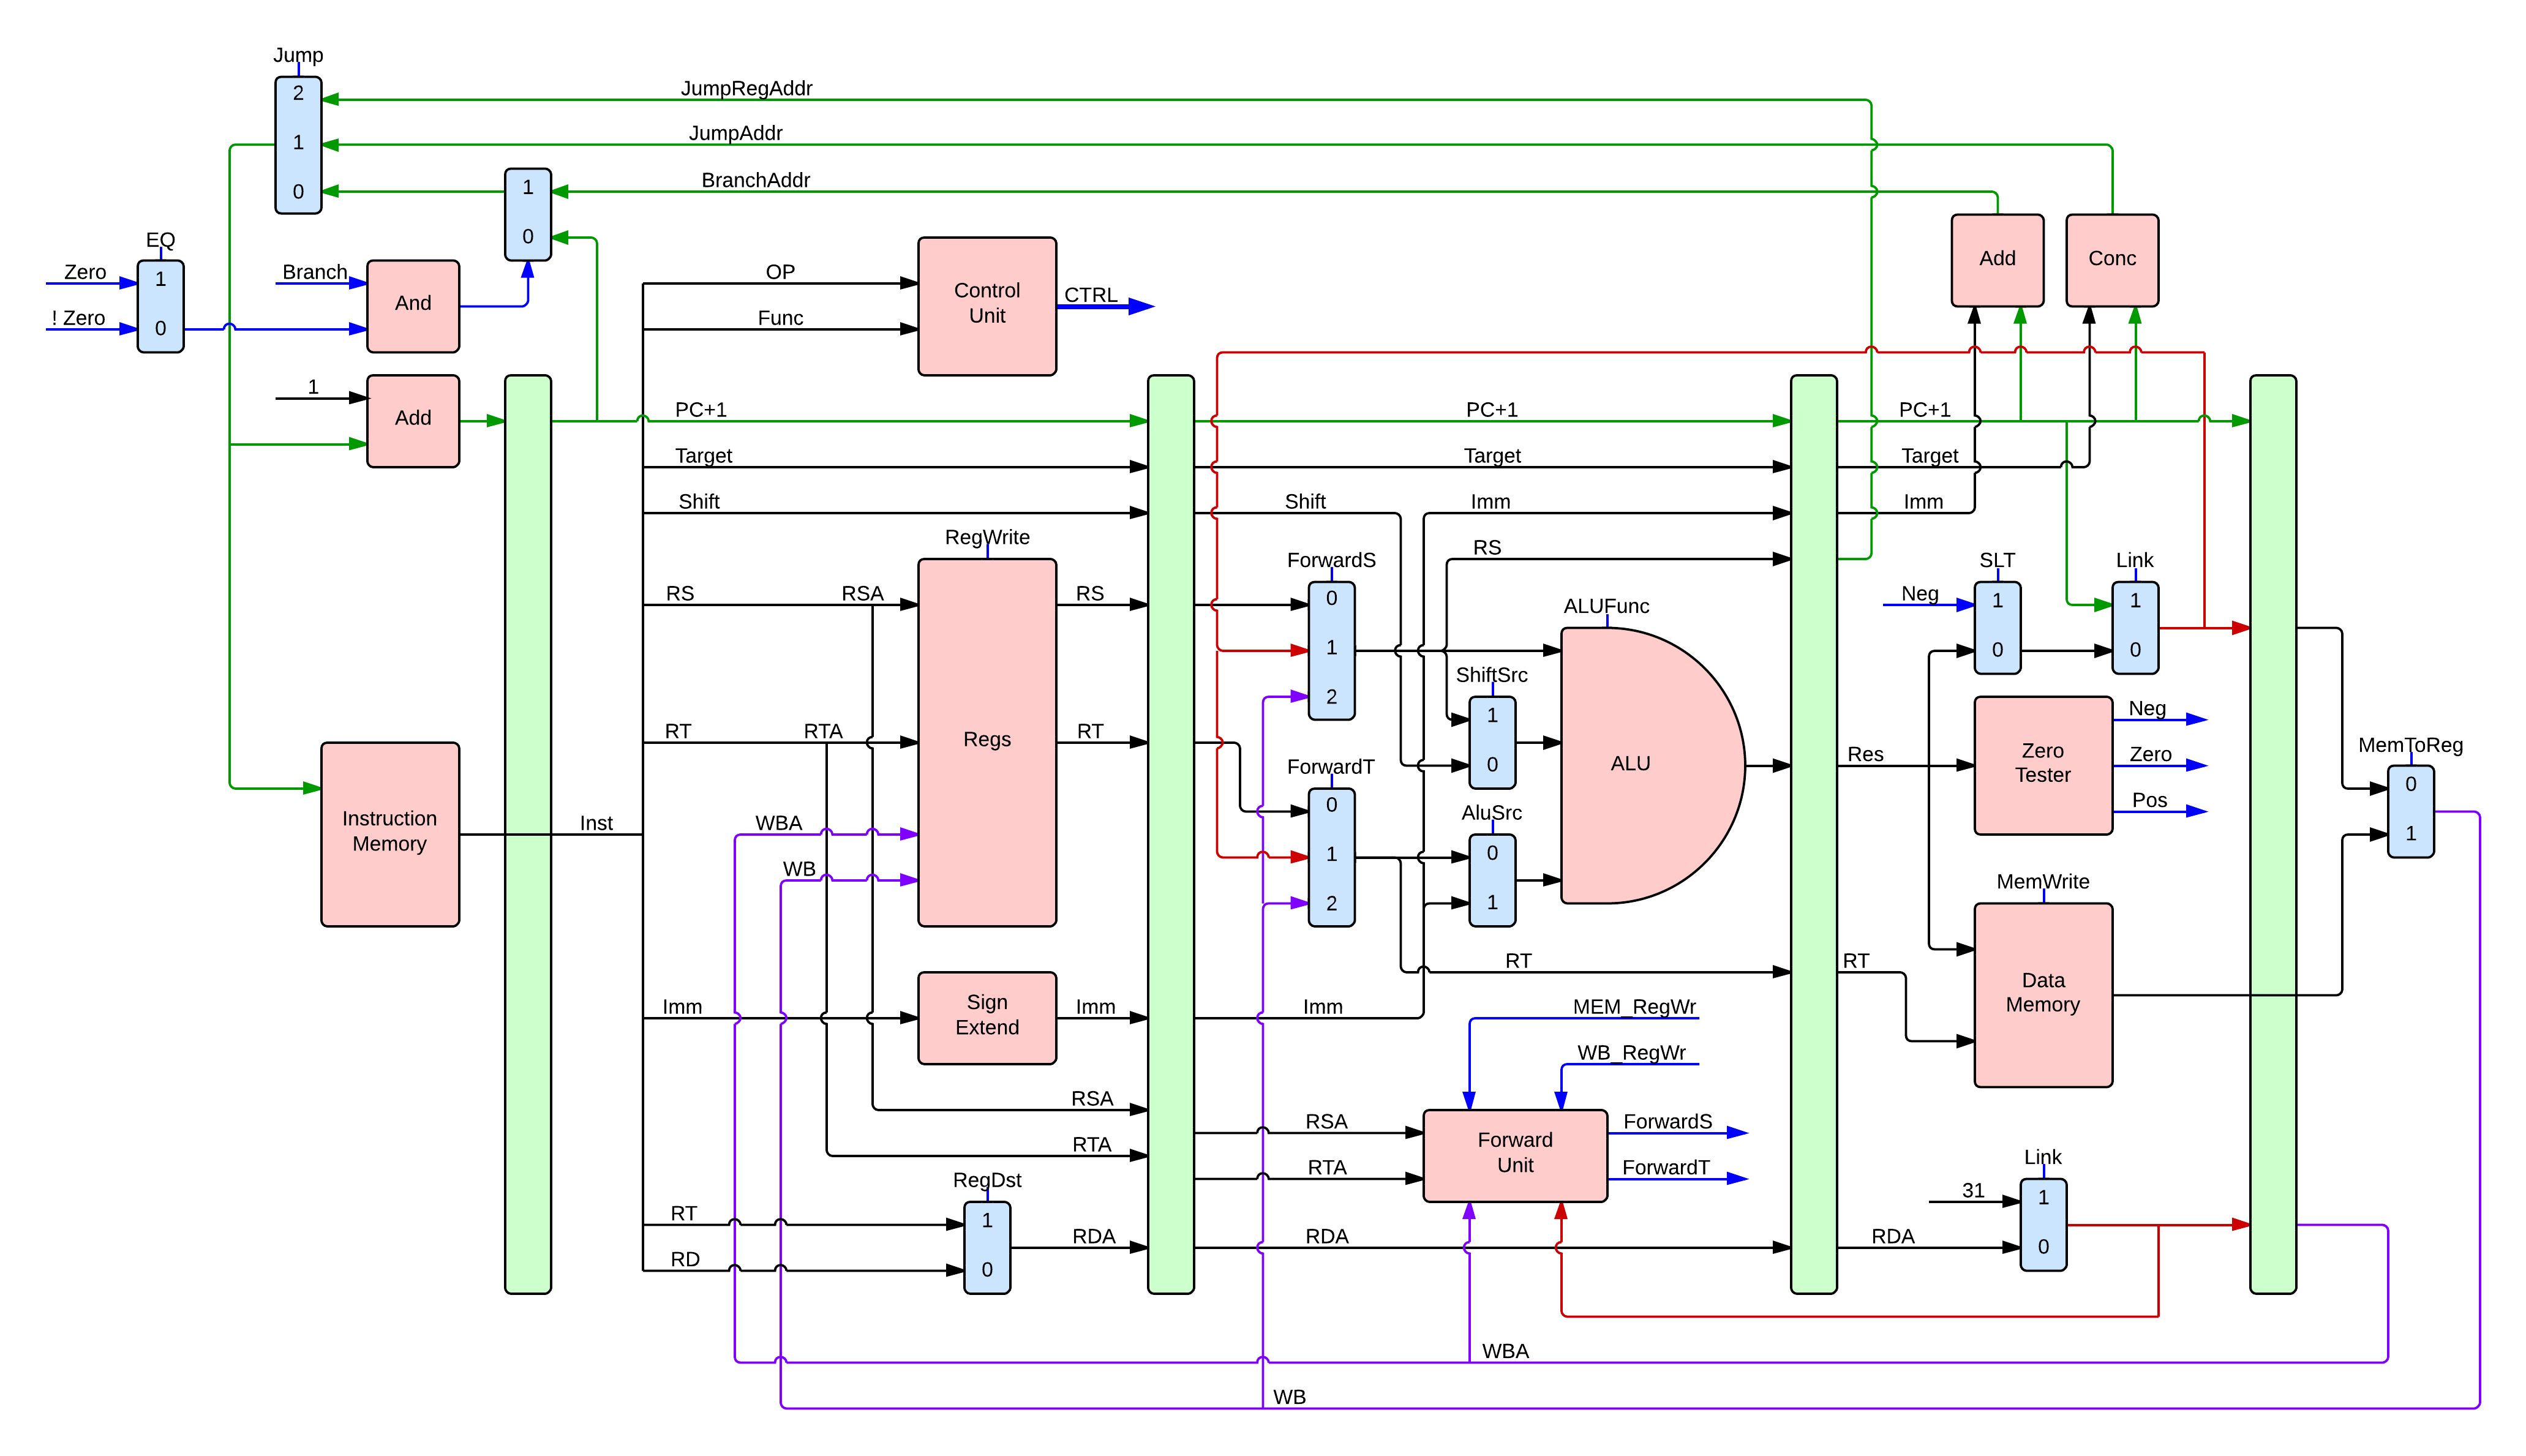
\includegraphics[width=\textwidth]{figures/Architecture.png}
    \caption{The implemented CPU architecture} 
    \label{fig:cpuArchitecture}
\end{figure}

There are a few things to note about this architecture.

First, since the instruction and data memories only read and write data on clock ticks, they act almost as pipeline registers for their own signals.
Therefore, their outputs are sent directly through the pipeline barrier to prevent the data from being delayed by an extra cycle.

Second, the address of the next instruction is fed directly into instruction memory to reduce latency, which allows the program counter to be merged into the first pipeline register.

Third, data from load word instructions is not forwarded from the memory stage and can therefore not be read in the following clock cycle.
This is a side effect of the data memory only acting on clock ticks.
Thus, to avoid reading invalid data, the instructions has to be reordered or a nop has to be added. This is normally accomplished by the assembler, which means it is hardly an issue.

\subsection{Instruction Set}

\subsection{Control Unit}

\subsection{Forwarding Unit}

\subsection{Branch Prediction}

